\section{Introduction}

Recently, Linux containers have drawn significant amount of attention because they are lightweight, portable, and repeatable.
Linux containers are generally more lightweight than virtual machine (VM) clusters, 
because the containers share the kernel with the host operating system (OS), even though they maintain separate execution environments. 
They are generally portable because the process execution environments are archived into tar files, 
so whenever one attempts to run a container, the exact same file systems are restored from the archives 
even when totally different data centers are used. 
This means that containers can provide repeatable and portable execution environments.
%
For the same reasons, Linux containers are attractive for web services as well, 
and it is expected that web services consisting of container clusters would be 
capable of being migrated easily for variety of purposes. For example disaster recovery, 
cost performance improvemets, legal compliance, and shortening the geographical distance to customers 
are the main concerns for web service providers in e-commece, gaming, Financial technology(Fintech) and Internet of Things(IoT) field.
%

Kubernetes\cite{K8s2017}, which is one of the popular container cluster management systems, 
enables easy deployment of container clusters.
Since Kubernetes hides the differences in the base environments, users can easily deploy a web service on different 
cloud providers or on on-premise data centers, without adjusting the container cluster configurations to the new environment. 
This allows a user to easily migrate a web service consisting of a container cluster even to the other side of the world. 
A user starts the container cluster in the new location, route the traffic there, 
then stop the old container cluster at his or her convenience.
This is a typical web service migration scenario.

However, this scenario only works when the user migrates a container cluster among major cloud providers including Google Cloud Platform (GCP), 
Amazon Web Services (AWS), and Microsoft Azure.
The Kubernetes does not include a load balancer, and is heavily dependent on external load balancers that are set up on the fly 
by cloud providers through their application protocol interfaces (APIs). 
These external load balancers distribute incoming traffic to every server that hosts containers.
The traffic is then distributed again to destination containers using iptables destination 
network address translation (DNAT)\cite{MartinA.Brown2017,Marmol2015} rules in a round-robin manner. 
The problem happens in the environment with a load balancer that is not supported by the Kubernetes, 
e.g. in an on-premise data center with a bare metal load balancer. 
In such environments, the user needs to manually configure 
the static route for inbound traffic in an ad-hoc manner. 
Since the Kubernetes fails to provide an uniform environment from a container cluster view point,
migrating container clusters among the different environments will always be a burden.

In order to solve this problem by eliminating the dependency on external load balancer,
we have proposed a containerized software load balancer that is run by Kubernetes as  
a part of web services consisting of container cluster in the previous work\cite{Takahashi2018}.

It enables a user to easily deploy a web service on different environment without modification, 
because the load balancer is included in the web service itself. 

We containerized Linux kernel's Internet Protocol Virtual Server (IPVS)\cite{Zhang2000} 
Layer 4 load balancer using an existing Kubernetes ingress\cite{K8sIngress2017} framework, as a proof of concept.
%
%
We also proved that our approach does not significantly deteriorate the performance,  
by comparing the performance of our proposed load balancer with those of 
iptables DNAT load balancer and the Nginx Layer 7 load balancing. 
%
The results indicated that the proposed load balancer could improve the portability of container clusters 
without performance degradation compared with the existing load balancer.

However, in our previous work, we have not discussed the redundancy of such load balancers.

Routing traffic to one of the load balancers while keeping redundancy in the container environment is a complex issue,
because standard Layer 2 rendandacy protocols, e.g. Virtual Router Redundancy Protocol(VRRP) or OSPF\cite{moy1997ospf} that uses multicast, 
can not be used in many cases.
Further more, providing uniform methods independent of various cloud environments and on-premise datacenter is much more difficult.   

In this paper we propose a software load balancer with ECMP redundancy for container cluster environment.

We containerize the linux kernels IPVS together with exabgp, and setup a redundant load balancer deployment using Kubernetes.
We also evaluate functionality and scalability of such a load balancer.


The contributions of this paper are as follows: 
1) We propose a portable software load balancer with ECMP redundacy as a part of a container cluster.
2) We demonstrate functionality of such load balancers using OSS networking softwares.
3) We also measure the performance of such load balancers.
4) Practical setups are demonstrated, and proven to function.

The rest of the paper is organized as follows.
Section \ref{Related Work} highlights work that deals specifically with container cluster migration, 
software load balancer containerization, and load balancer related tools within the context of the container technology. 
Section \ref{Load balancers in Kubernetes cluster} will explain existing architecture problems and propose our solutions.
In Section \ref{Performance Measurement}, experimental conditions and the parameters 
that we considered to be important in our experiment will be described in detail.
Then, we will show our experimental results and discuss the obtained performance characteristics in Section~\ref{Result and Discussion},  
which is followed by a summary of our work in Section~\ref{Conclusions}.

\section{Related Work}\label{Related Work}

This section highlights related work, especially that dealing with container cluster migration, 
software load balancer containerization, load balancer tools within the context of the container technology and scalable load balancer in the cloud providers.

\paragraph{\bf Container cluster migration:}

Kubernetes developers are trying to add federation\cite{K8sFederation2017} capability for handling situations 
where multiple Kubernetes clusters\footnote{The {\em Kubernetes cluster} refers to a server cluster 
controlled by the Kubernetes container management system, in this paper.} 
are deployed on multiple cloud providers or on-premise data centers, 
and are managed via the Kubernetes federation API server (federation-apiserver). 
However, how each Kubernetes cluster is run on different types of cloud providers
and/or on-premise data centers, especially when the load balancers of such environments are not supported by Kubernetes, 
seems beyond the scope of that project. 
The main scope of this paper is to make Kubernetes usable in environments 
without supported load balancers by providing a containerized software load balancer.

\paragraph{\bf Software load balancer containerization:}
As far as load balancer containerization is concerned, the following related work has been identified:
Nginx-ingress\cite{Pleshakov2016,NginxInc2016} utilizes the ingress\cite{K8sIngress2017} capability of Kubernetes, 
to implement containerized Nginx proxy as a load balancer. Nginx itself is famous as a high-performance web server program
that also has the functionality of a Layer-7 load balancer. Nginx is capable of handling Transport Layer Security(TLS) encryption, 
as well as Uniform Resource Identifier(URI) based switching. However, the flip side of Nginx is that it is much slower than Layer-4 switching.
We compared the performance between Nginx as a load balancer and our proposed load balancer in this paper.
%
Meanwhile, the kube-keepalived-vip\cite{Prashanth2016} project is trying to use Linux kernel's IPVS\cite{Zhang2000} 
load balancer capabilities by containerizing the keepalived\cite{ACassen2016}.
The kernel IPVS function is set up in the host OS's net name spaces and is shared among multiple web services,
as if it is part of the Kubernetes cluster infrastructure.
Our approach differs in that the IPVS rules are set up in container's net name spaces 
and function as a part of the web service container cluster itself.
The load balancers are configurable one by one, and are  movable with the cluster once the migration is needed.
The kube-keepalived-vip's approach lacks flexibility and portability whereas ours provide them.
%
The swarm mode of the Docker\cite{DockerCoreEngineering2016,DockerInc2017} also uses IPVS for internal load balancing,
but it is also considered as part of Docker swarm infrastructure, 
and thus lacks the portability that our proposal aims to provide.

\paragraph{\bf Load balancer tools in the container context:}
There are several other projects where efforts have been made to utilize IPVS in the context of container environment.
For example, GORB\cite{Sibiryov2015} and clusterf\cite{Aaltodoc:http://urn.fi/URN:NBN:fi:aalto-201611025433} are daemons 
that setup IPVS rules in the kernel inside the Docker container. 
They utilize running container information stored in key-value storages
like Core OS etcd\cite{CoreOSEtcd} and HashiCorp's Consul\cite{HashiCorpConsul}. 
Although these were usable to implement a containerized load balancer in our proposal, we did not use them, 
since Kubernetes ingress framework already provided the methods to retrieve running container information through standard API.

\paragraph{\bf Cloud load balancers:}

As far as the cloud load balancers are concerned, two articles have been identified.
Google's maglev\cite{eisenbud2016maglev} is a software load balancer used in Google Cloud Platform(GCP)\cite{Voellm2013}.
Maglev uses modern technologies including per flow ECMP and kernel bypass for userspace packet processing.
Maglev serves as the GCP's load balancer that is used by the Kubernetes.
Maglev can be solely used in GCP, and the users need open source software load balancer that is runnable even in on-premise data centers.
Microsoft's Ananta\cite{patel2013ananta} is another software load balancer implementation using ECMP and windows network stack.
Ananta can be solely used in Microsoft's Azure cloud infrastructure\cite{patel2013ananta}.
The proposed load balancer by the author is different in that it is aimed to be used in every cloud provider and on-premise data centers.

\section{Proposed Architecture}\label{Architecture}
\subsection{Basic Architecture of Kubernetes Cluster}
Discuss K8S LB architecture

\subsection{Overlay network}
Since the knowledge of the overlay network is important to setup redundant load balancers, 
we briefly explain an abstract concept of overlay network that is common to existing overlay network including flannel and calico.

\begin{figure}
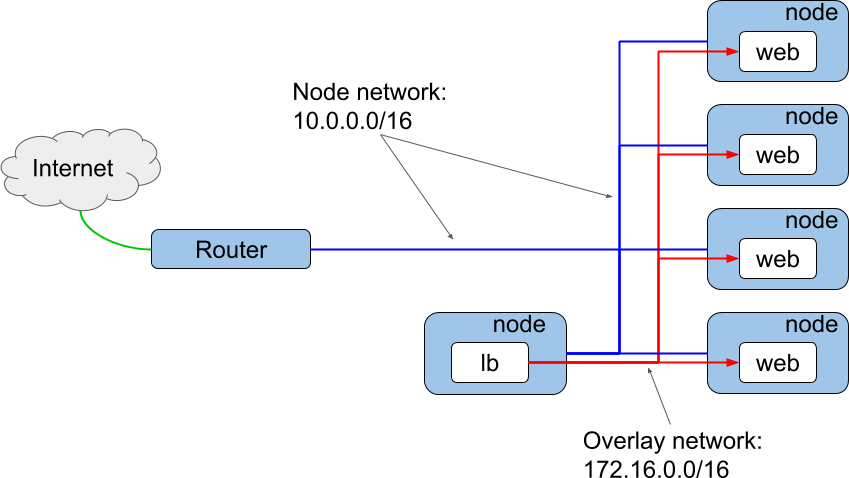
\includegraphics[width=\columnwidth]{Figs/overlay.png}
\caption{Network architecture of an exemplified container cluster system. An overlay networks is .... }
\label{fig:overlay}
\end{figure}

Figure~\ref{fig:overlay} shows schematic diagram of network architecture of a container cluster system. 

An overlay network consists of appropriate routing tables on nodes, optionally tunneling using ipip or vxlan.
 
The overlay network is the network for containers to communicate with each other. The node network is the network for nodes to communicate with each other.

When the ipvs container in the Fig.1 communicates with the other nodes, the nodes can properly route the packets because they have the routes to 172.16.0.0/16 in their routing table, which is a part of overlay network setups.

When a container in the Fig.1 communicates with the router, packets from 172.16.0.0/16 network are translated by SNAT setup on each node.

\subsection{ECMP redundancy in container network}
 
\begin{figure}
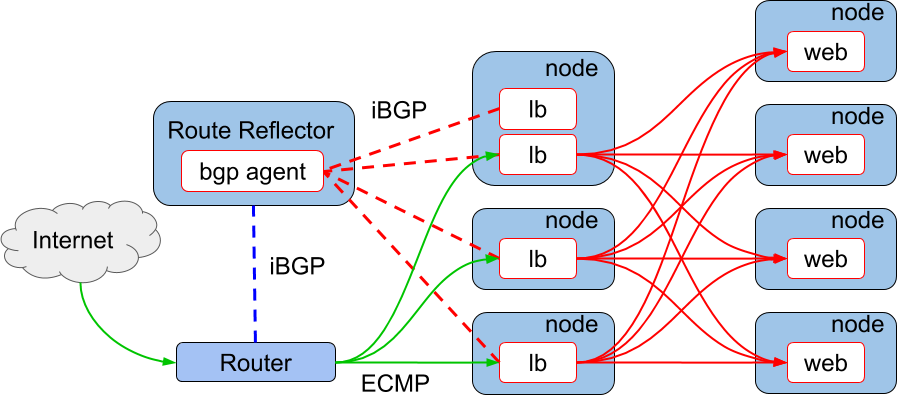
\includegraphics[width=\columnwidth]{Figs/ecmp.png}
\caption{Network architecture of an exemplified container cluster system. An overlay networks is .... }
\label{fig:ecmp}
\end{figure}

Figure~\ref{fig:ecmp} shows our poroposed redundancy architecture for software load balanceer.

Since the router has no knowledge of overlay network, the communication between the router and ipvs containers have to be via SNAT.
If we were to setup BGP peering directly between containers and the router, such connections are between a node’s IP address and the router’s. 
In such cases, the router might not be able to set up multiple BGP session from a single node.

In other to alleviate this, we used a node with the knowledge of overlay network as a route reflector. 
Since the communication between the route reflector and ipvs containers are between the node network IPs and overlay network IPs, 
the route reflector can accept sessions from multiple ipvs containers on a single node.    

\begin{figure}
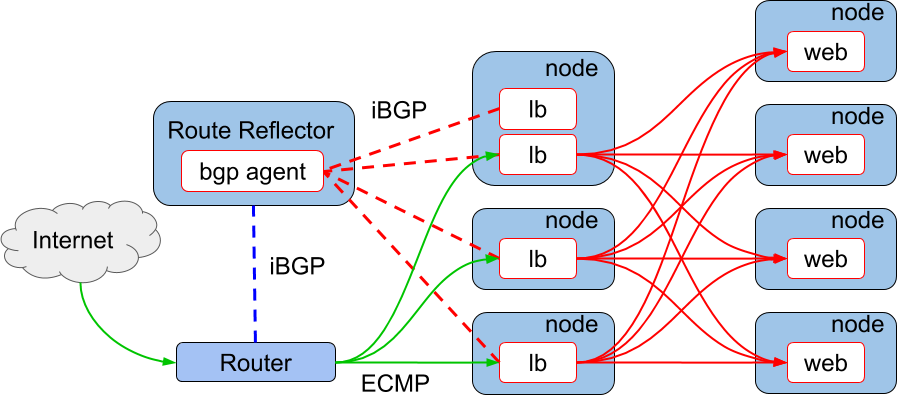
\includegraphics[width=\columnwidth]{Figs/ecmp.png}
\caption{Network architecture of an exemplified container cluster system. An overlay networks is .... }
\label{fig:vrrp}
\end{figure}

Figure~\ref{fig:vrrp} shows VRRP redandancy as a comparison.


ECMP is better.

\section{Implementation}\label{Implementation}

\subsection{IPVS containerization}


\subsection{BGP software containerization}

\subsection{Proof of concept system architecture}


\section{Evaluation}\label{Evaluation}

\subsection{Functionality}\label{Functionality}

\subsubsection{Redundancy}

\subsubsection{Load balancing}

\subsection{Performance}\label{Performance}



\section{Conclusions}\label{Conclusions}

In this paper, we proposed a portable software load balancer that has the following features, 1) runnable as a Linux container, 2) redundancy with ECMP technique,  for the container cluster systems.

Our load balancer aims at facilitating migration of container clusters for web services.
We implemented a containerized software load balancer that is run by Kubernetes as a part of container cluster,
using Linux kernel's IPVS.

To discuss the feasibility of the proposed load balancer, we built
a Kubernetes cluster system and conducted performance measurements.
Our experimental results indicate that the IPVS based load balancer in container improves the portability of
the container cluster while it shows the similar performance levels as the existing iptables DNAT based load balancer.

We also started to the implementation of a novel software load balancer using recently introduced Linux kernel's XDP infrastructure.
While it is in a preliminary stage of the development, essential functions and design issues have been already clarified.
They will be presented at the time of the presentation.

\section{Future work}\label{Future work}

We leave the following for the future work:
1) Performance measurement of XDP load balancer
2) Implementation of consistent hashing balancing algorithm
3) Containerization of XDP load balancer
These works are ongoing and will be presented when they are available.

